\section{Secure User Interaction}


\myparagraph{Motivation} A user communicates with a remote server through a \emph{host} system that is typically a standard PC (specifically $x86$ architecture), which gives the host access to the raw IO data that is exchanged between the user and the remote server. The host consists of large and complex system software such as the operating system, device drivers, applications such as browser, and a diverse set of hardware components that expose the host to a large attack surface. An adversary that controls the user's host can alter user intentions, i.e., it can perform arbitrary actions on behalf of the user, modify the input parameters, or show wrong information to the user. Such an adversary is very powerful and difficult to be detected or prevented by a remote server. Hence, existing defense standards for web UI are ineffective as the browser is untrusted also. The consequences of such attacks might be severe when applications that control remote safety-critical systems are targeted. The attacker can pass the wrong input to a remote safety-critical system such as a medical device, power plant, etc., or leak sensitive information such as credentials for e-banking, candidate preference in the e-voting, etc.


\myparagraph{Trusted path} Trusted path provides a secure channel between the user (specifically human interface device - HID) and the end-point, which is typically a trustworthy application running on the host. Trusted path ensures that user inputs reach the intended application unmodified, and all the outputs presented to the user are generated by the legitimate application. Trusted path to the local host is a well-researched area where many solutions focus on using trusted software components such as a trusted hypervisor. Zhou et al.~\cite{zhou2012building} proposed a generic trusted path on $x86$ systems with a pure hypervisor-based design. SGXIO~\cite{weiser2017sgxio} employs both a hypervisor and Intel SGX. However, hypervisors are hard to deploy, have a large TCB, and are impractical in real-world scenarios as most of the existing verified hypervisors offer a minimal set of features.

\subsection{Limitations in the Current TEE}

The recent introduction of trusted computing architectures like Intel's SGX has enabled secure computations and secure data storage on otherwise untrusted computing platforms. However, such architectures do not directly enable secure user interaction because IO operations are handled by the operating system. Additionally, the recent microarchitectural attacks have shown that execution environments inside enclaves, like the one provided by SGX, can be compromised as well.


\subsection{Requirements of Security \& Functional Properties}
\label{goals}

The lack of security properties and features in the existing solutions provides the necessary security and functional requirements for a trusted path that provides IO integrity and confidentiality and is usable. We can now summarize the observations that we derived from the literature as following:

\myparagraph{R1. Inter-dependency between input and output} 
IntegriKey~\cite{IntegriKey} use external embedded devices to sign input parameters. However, such solutions do not support output integrity; hence, the attacker can execute UI manipulation attacks to trick the user into providing incorrect inputs. Such observation shows that the output and input security depend on each other, and they should be considered together. Otherwise, the attacker can manipulate the output to influence the user input.
%The main lesson that we learn from the previous papers is that input and output integrity, and confidentiality cannot be considered in isolation. Rather, they are needed to be secured simultaneously as the output, and the input both influence each other.  

\myparagraph{R2. Inter-dependency between all input modalities} 
Fidelius~\cite{Fidelius} combines the previous ideas of Bump in the Ether and trusted overlay to protect keyboard inputs from a compromised browser using external devices and a \js interpreter that runs inside an SGX enclave. However, not supporting mouse causes Fidelius to susceptible to early form submission attack where the attacker could maliciously submit a form when the user is still typing - violation of input integrity. Existing web interfaces allow users to complete forms by using different modalities for the user input, namely the keyboard, the mouse, and the touchpad. The observation from Fidelius secure shows that system should protect simultaneously all user input modalities to achieve input integrity (against early-form submission and clickjacking).


\myparagraph{R3a. No cognitive load for IO integrity} 
A system that protects IO operations should introduce minimal or no cognitive load to its users for input integrity.
The system should guarantee the output integrity of the legitimate information necessary to complete a form and avoid asking the user to interact with an external device or monitor security indicators out-of-context.


\myparagraph{R3b. User attention for IO confidentiality} Preserving the confidentiality of user inputs against a compromised host is a challenging task because the host can trick the user to reveal her inputs when the system is not active. Therefore, requiring users to perform a small action, e.g., press a key, before entering confidential inputs is a valid trade-off between usability and security.

%Confidentiality requires active triggering from the user to distinguish the secure part of the screen from ensuring part of the screen if the part of the output provides integrity/confidentiality protection.

\myparagraph{R4. Small trust assumptions and deployability} 
Our goal is to provide the rich set of IO and security features with minimal trust assumptions that do not rely on a trusted OS, specialized hypervisor, or TEEs such as Intel SGX. Preferably, the solution should be easy to set up for users, i.e., plug-and-play, and integrate well with the existing infrastructure.  


\subsection{High-level Description of \name}

\begin{figure}[t]
\centering
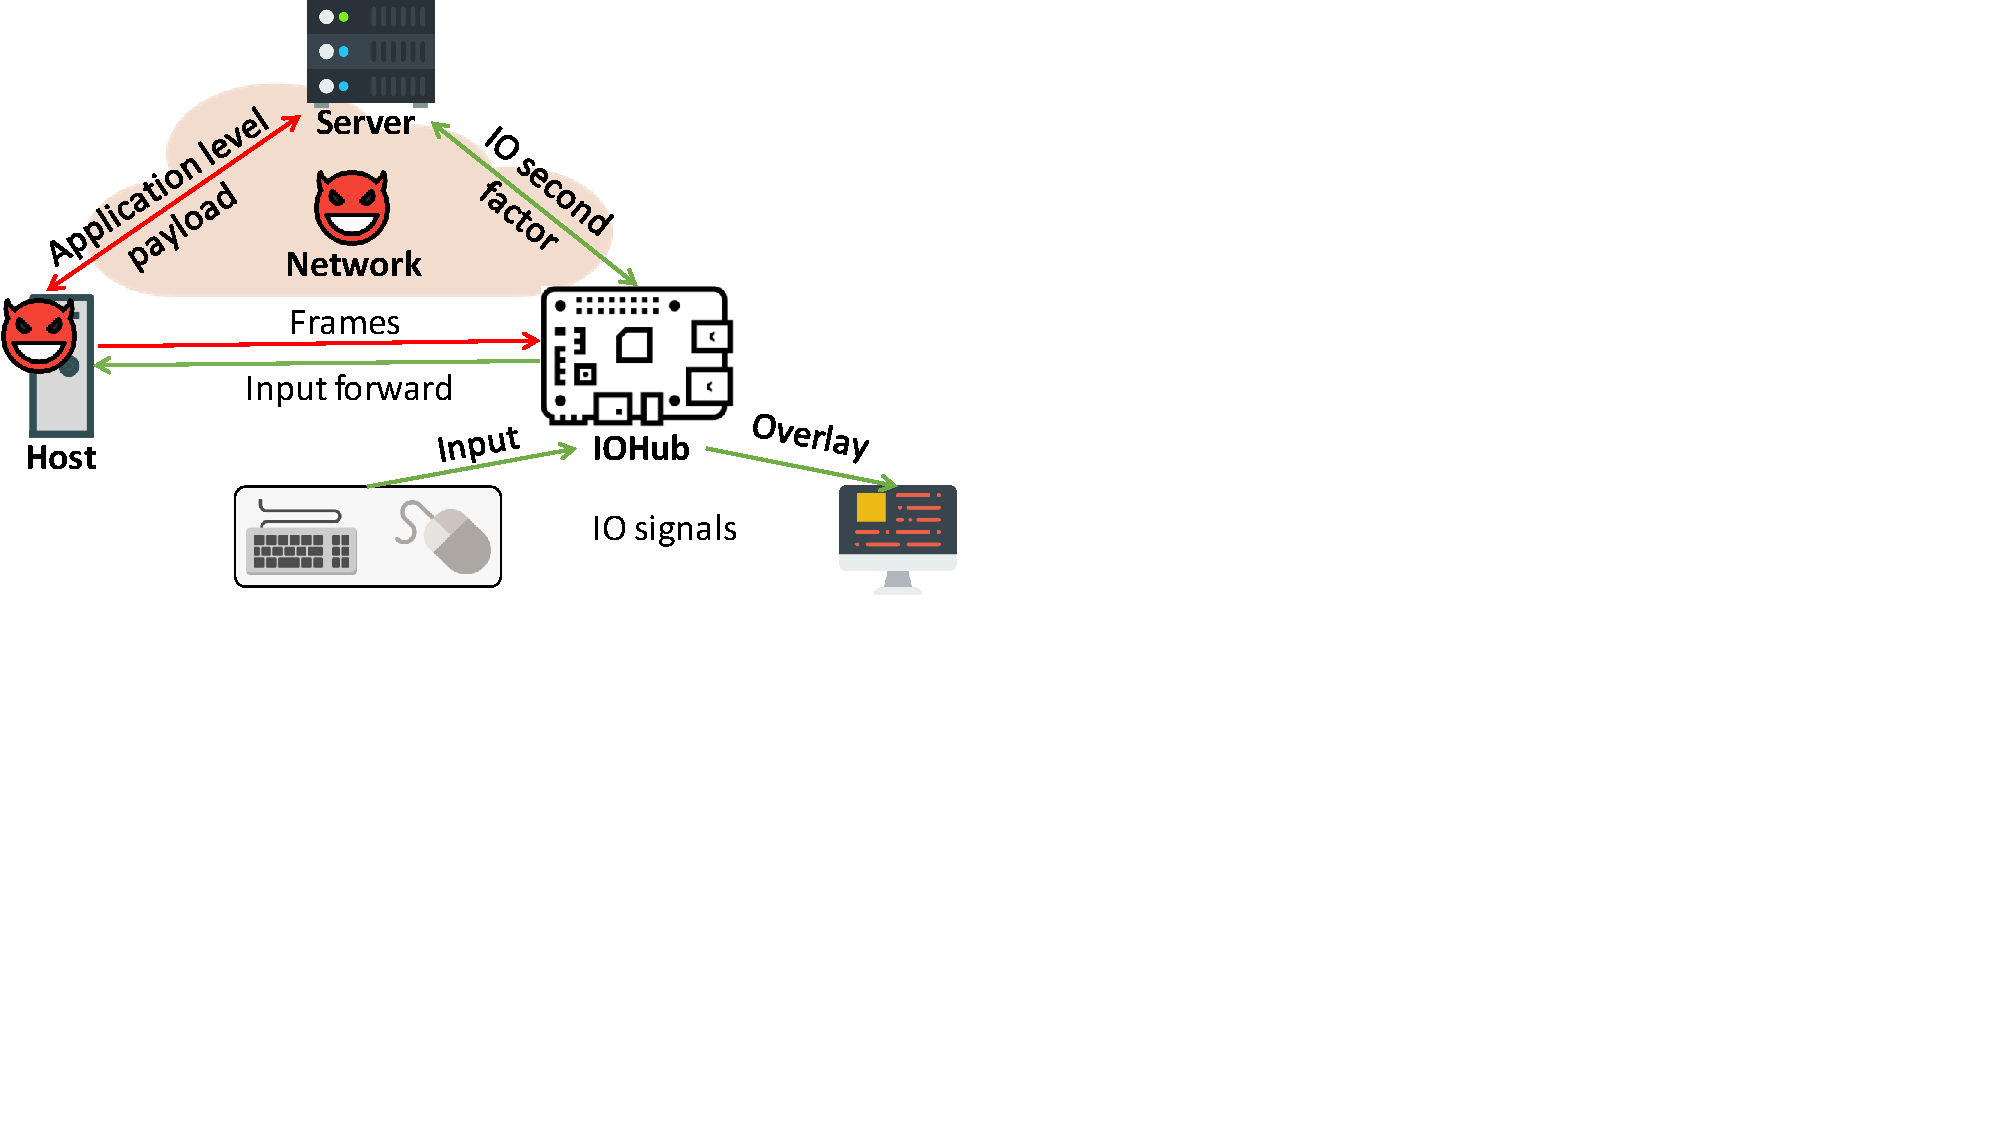
\includegraphics[trim={0 8.5cm 17cm 0}, clip, width=0.85\linewidth]{approachOverview.pdf}
\caption{\textbf{High-level approach overview of our solution.}  The \device connects the trusted IO devices and the attacker-controlled host. 
}
\spacesave
\label{fig:approachOverview}
\centering
\end{figure}


\begin{figure}[t]
\centering
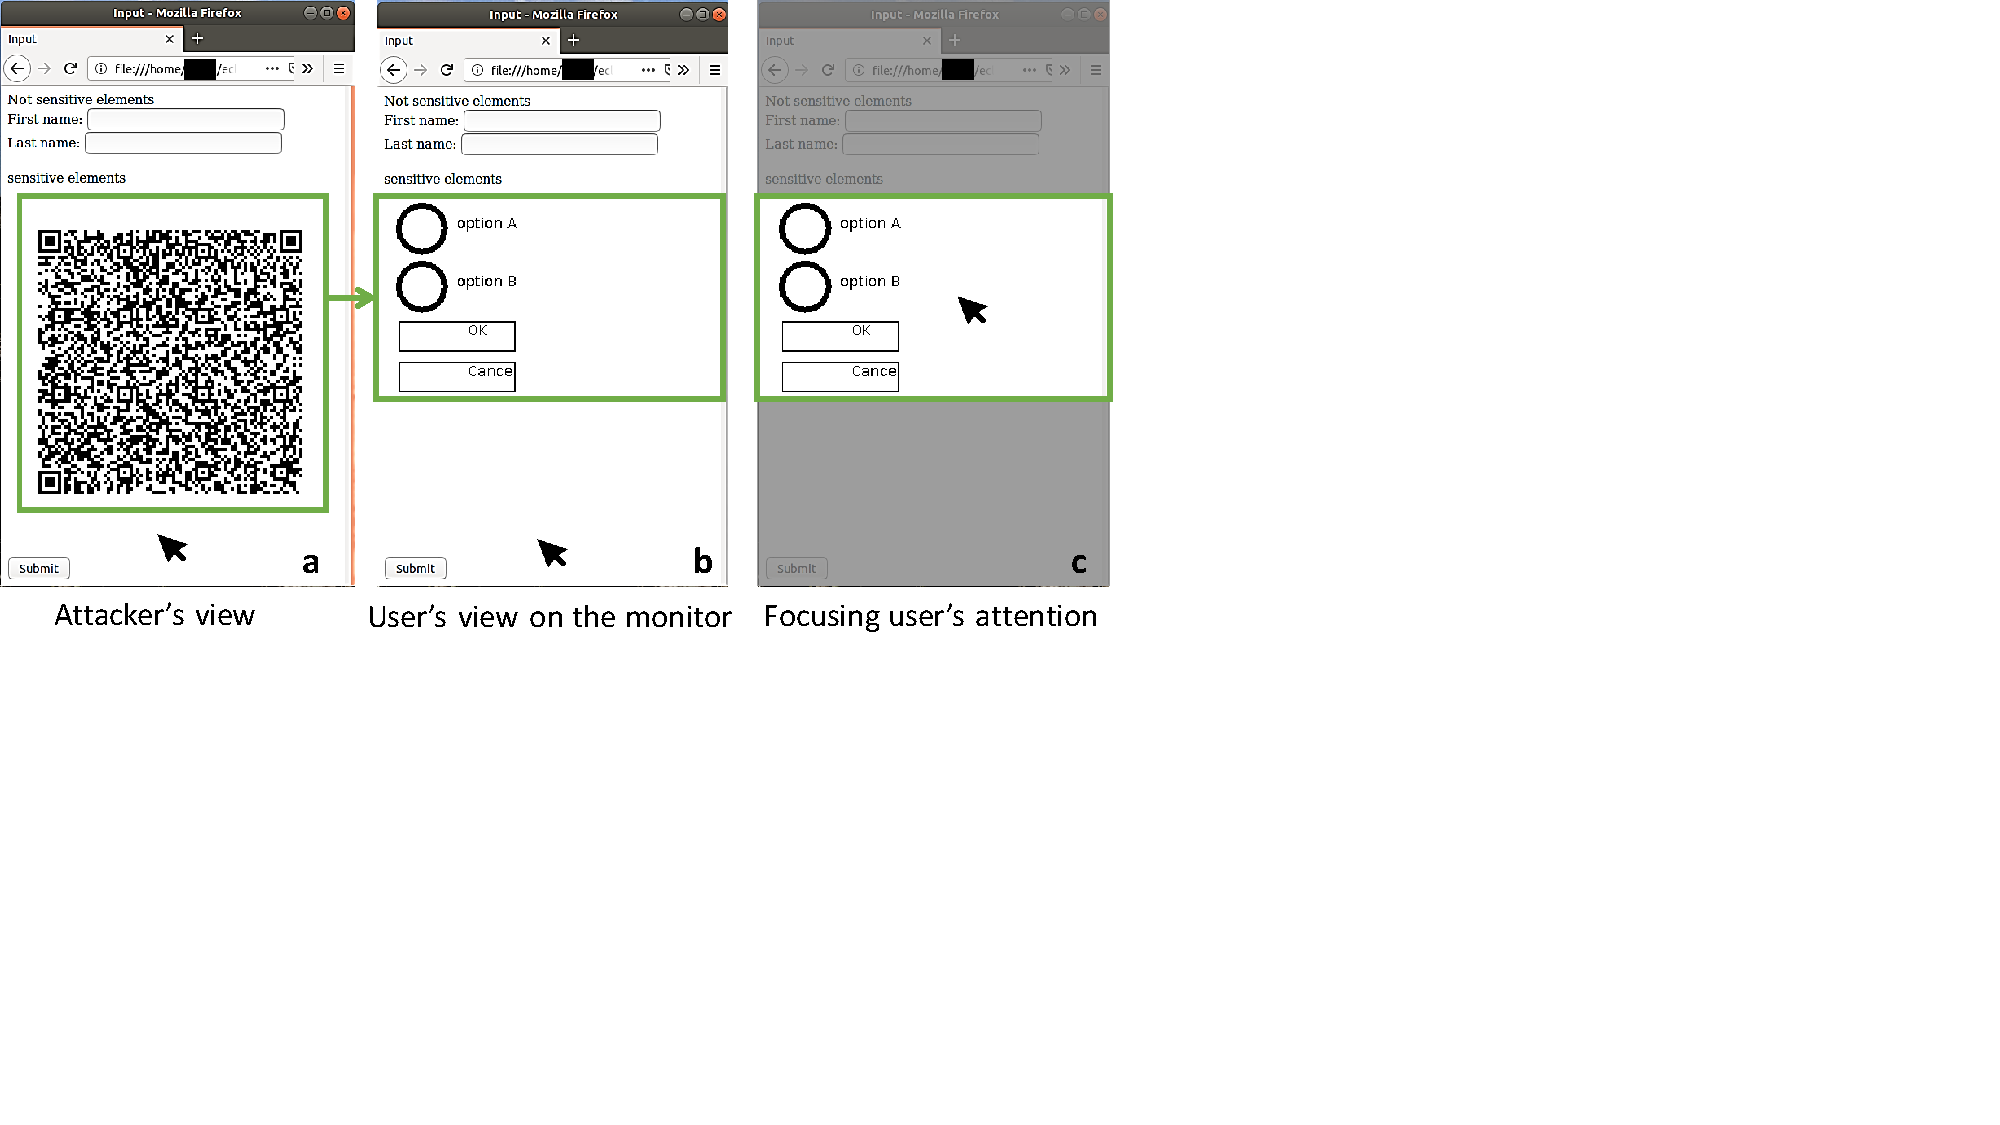
\includegraphics[trim={0 8cm 15cm 0}, clip, width=\linewidth]{overlayScreenShot_new.pdf}
\caption{\textbf{\name's high-level approach} shows that the \device generates UI overlay to protect IO integrity and confidentiality. a) The attacker only sees the non-protected UI elements, and the protected form is encrypted and encoded (in our case, the \device could decode a QR code and decrypt). b) shows the \device generated form overlay that is hidden from the host. The protected part of the screen provides integrity and confidentiality of all user IO. c) shows that the \device dims out (lightbox) the rest of the screen when the user moves her mouse pointer over the protected region to focus user attention.}
\spacesave
\label{fig:screenshot_1}
\end{figure}

We consider a typical scenario where the user wants to interact with a trusted remote web server via an attacker-controlled host. The model is depicted in Figure~\ref{fig:approachOverview} which shows the untrusted host, the remote server, and the user IO devices. We only assume that the monitor, keyboard, mouse (in a word all the IO devices that we need to protect from the malicious host) and the \device are trusted. The \device works as a mediator between all the IO devices and the host. Note that the \device has no network capability to communicate with the server directly, rather it relies on the host and uses it as an untrusted transport. We also assume that the \device comes with preloaded certificates and keys that allow the \device to verify the signatures signed by the server and sign data such as the user input.

There are many possible ways to deploy \name. One way is to assume that the \device manufacturer issues a certificate for each of the deployed \device{}s . The \device maintains a whitelist for the remote servers along with their public certificates. This allows the \device to verify messages signed by those remote servers. Another assumption could be that the \device is issued by a service provider who also runs the remote server. 


\myparagraph{Attacker model and capabilities} Our attacker model assumes that the host (OS, installed applications, and hardware) and the network are attacker-controlled. The attacker can intercept, and arbitrarily manipulate (such as create, drop, or modify) the user IO data between the user and the remote server. Furthermore, we assume that the attacker can not break the physical security of the \device.

\name is build upon the security requirements and functional properties that are described in Section~\ref{goals}. 
\device is active only when the user visits sensitive web applications that require \name security.
Initially, the remote server signs and delivers the sensitive UI elements to the host in a format that is understandable by \device. Next, the host transfers the sensitive UI to \device, and the \device verifies the signature to prevent manipulations by the host. As seen in a running example depicted in Figure~\ref{fig:screenshot_1}, the \device then renders the UI with sensitive elements into an overlay on top of the HDMI frame received from the host. Note that the host cannot access or modify the overlay generated by the \device. Also, the overlay covers only a part of the screen, allowing the other feature-rich content on the webpage to run unmodified. Therefore, this ensures that sensitive UI elements are presented to the user as expected by the remote server -- \emph{output integrity}. For the overlay, we use QR-codes to transfer data from the host to the device because we avoid using extra software/hardware for a separate channel, and it is easy to visualize.

When the user interacts (types or moves the pointer) with the overlay, \device does not forward any event from the keyboard or the mouse to the host. The interaction is maintained solely by \device, which renders on-screen user inputs and therefore offers a user experience that is identical to a typical one as if the \device is not present. The user click on the \emph{submit} button triggers the submission procedure, which consists of the \device signing the user inputs and sending to the server. Note that the text fields of the form and the \emph{submit} button are inside the overlay which is inaccessible by the host, hence the attacker cannot execute the early form submission or clickjacking attacks. Finally, the server verifies the signature of \device to guarantee that the host has not altered the data. Therefore, the \device ensures \emph{input integrity} for all \emph{modalities} of input.

For integrity guarantees, \name uses well-known user attention focusing mechanisms. Unlike systems like Fidelius, these mechanisms do not introduce any cognitive load to the users as \name does not rely on multiple security indicators. Mechanisms such as lightbox aid the user to distinguish the \device overlay on the screen from the rest. Thus, the untrusted host cannot trick the user into following malicious instructions when the user interacts with sensitive UI elements. Also, the host cannot observe sensitive data on the overlay because it does not have access to it. In the case where confidentiality is required, the user manually triggers SAS, such as the lightbox by pressing specific keys.


\begin{figure}[t]
\centering
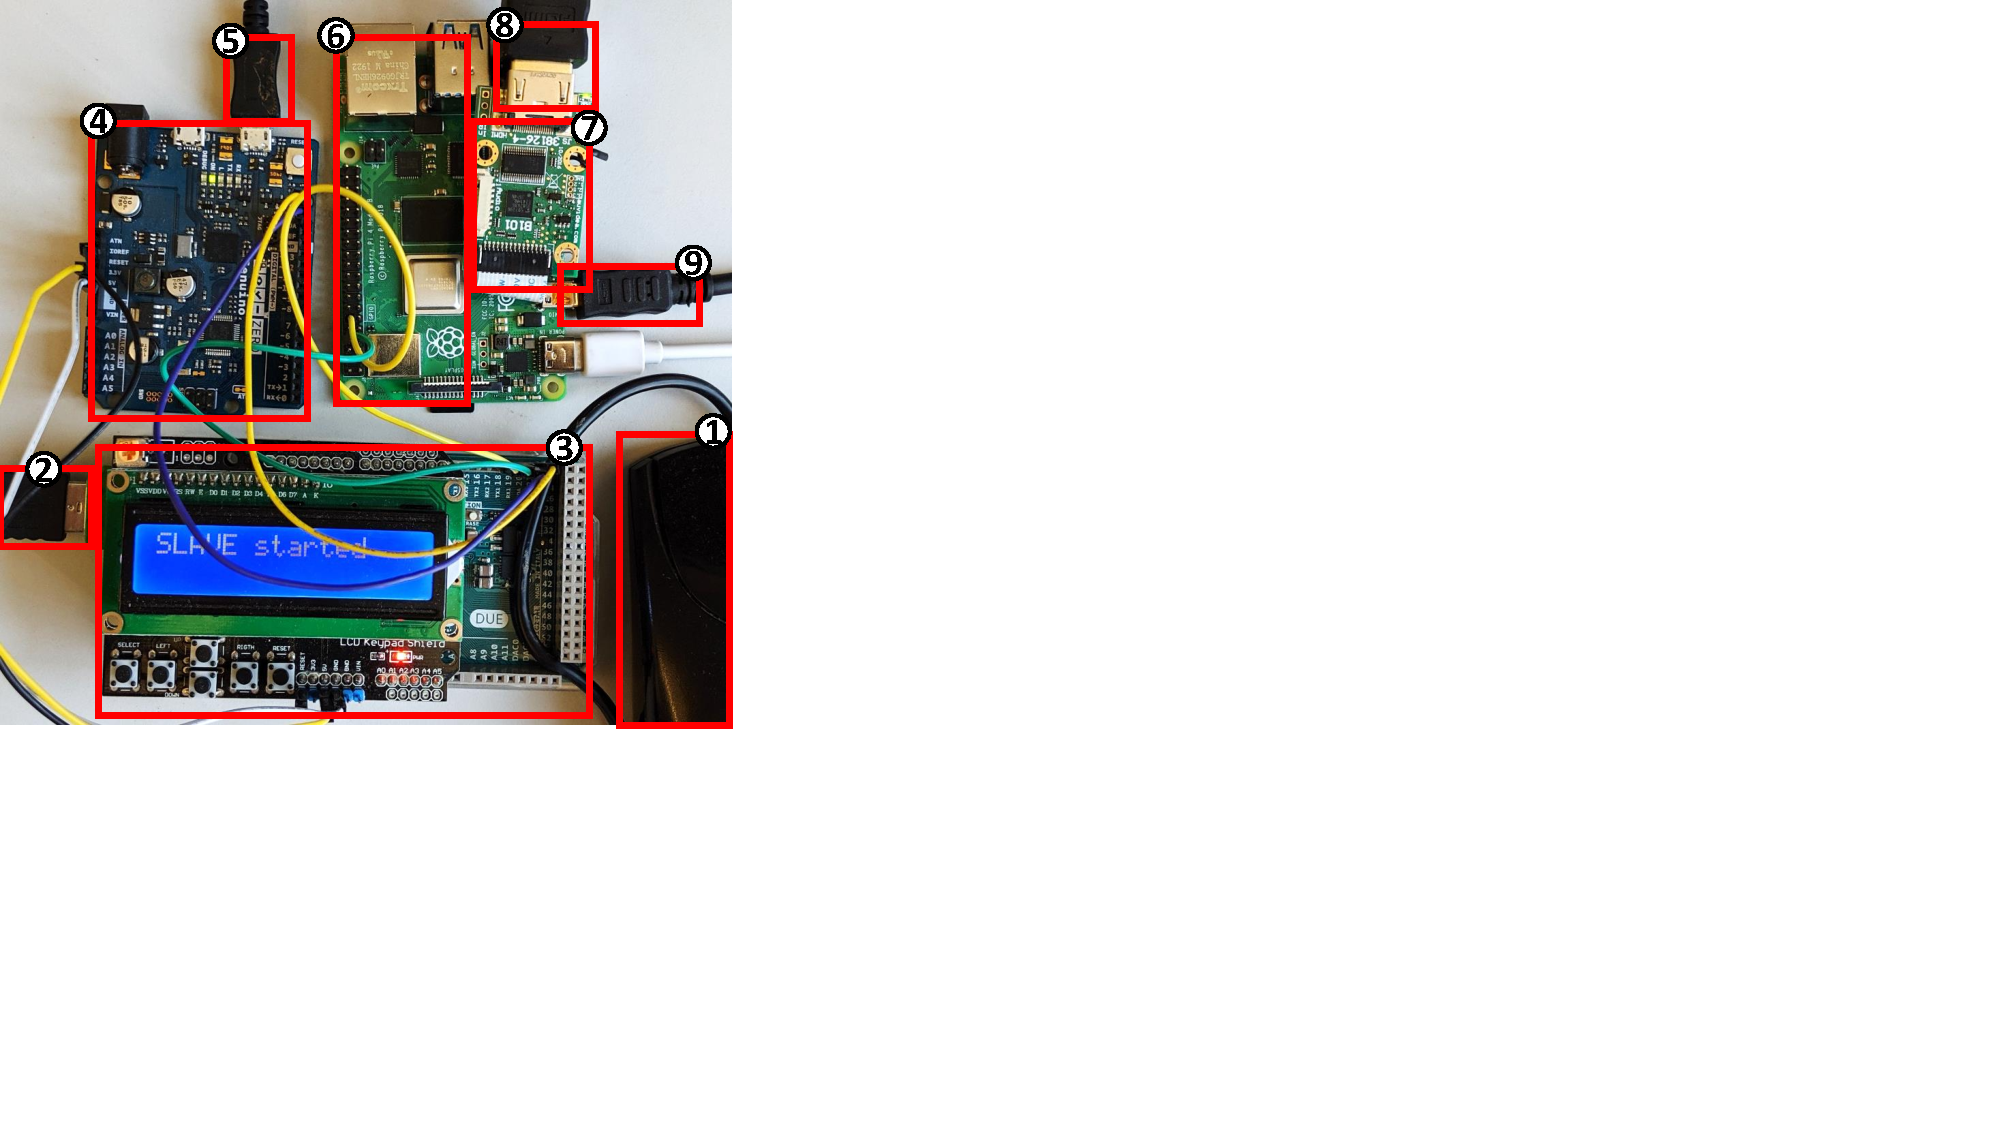
\includegraphics[trim={0 6.6cm 21.5cm 0}, clip, scale=0.55]{setUp_1.pdf}
\caption{The figure shows \name prototype that employs Arduino Due and Zero microcontroller board and a Raspberry Pi 4 SBC.}
\label{fig:prototypeArch}   
\end{figure}

\subsection{Prototype and Evaluation}

Figure~\ref{fig:prototypeArch} shows our \device prototype. We evaluate the performance of our prototype by measuring the overheads introduced by \name to the system and whether they influence the user's interaction. Initially, we measure the default latency introduced by \device when the user interacts with applications that do not require protection.
The delay in forwarding keystrokes is $170\ \mu s$ and for frames is $21.76\ ms$. This allows the \device to achieve the maximum display frame rate of $47.69$ per second (e.g., most of the movies are shot and shown in  ~24-30 fps). However, an optimized implementation of the technique to encode information in the HDMI frame would reduce significantly the processing time of a frame and increase further the frame rate as a result. Note that the B101 HDMI to CSI board that we use to intercept HDMI, has a hardware limit of 25 frames at 1080p resolution.







